\documentclass[11pt]{beamer}

\RequirePackage{silence}
\WarningFilter{remreset}{The remreset package}

\usetheme{Copenhagen} %metropolis#
\useoutertheme{infolines}
\usecolortheme{default}

%%%%%%%%%%%%%%%%%%%%%%%%%%%%%%%%%%%%%%%%%%%%%%%%%%%%%%%%%%%%%%
%
% 1. Personendaten
%
\author[Diener, Roob, B{\'e}k{\'e}si]
{Irene~Diener, Toni~Roob, Jarod~A.~M.~B{\'e}k{\'e}si}
\newcommand{\myTitle}{Einf{\"u}hrung in die Quantenkommunikation}
\newcommand{\myTitleShort}{Quantenkommunikation}
\title[\myTitleShort]{\myTitle}
%\subtitle{}
\newcommand{\myProf}{Prof.~Dr.~habil.~Andriy~Luntovskyy}
\newcommand{\myAcademy}{Duale Hochschule Sachsen}
\newcommand{\myStudy}{Studiengang Informationstechnik}
\newcommand{\myLocation}{Dresden} 
\newcommand{\myVersion}{Version 1.0}
% Abgabedatum
\newcommand{\mySubmissionDate}{30. September 2025}


%%%%%%%%%%%%%%%%%%%%%%%%%%%%%%%%%%%%%%%%%%%%%%%%%%%%%%%%%%%%%%
%
% 2. Packete
%
\usepackage[latin1]{inputenc}
\usepackage[T1]{fontenc}
\usepackage{lmodern}

\usepackage{hyphenat}
\usepackage[ngerman,english]{babel}
\usepackage[babel]{csquotes}
\usepackage{cite}
\usepackage{amsmath,amssymb,amstext,amsthm}
\usepackage{upgreek,units}

\usepackage{ragged2e}
\usepackage{animate}

\usepackage{graphicx}
\usepackage{caption,subcaption}

\usepackage[hang,multiple]{footmisc}
\renewcommand{\footnotemargin}{1.2em}
\usepackage{longtable,booktabs,multirow,colortbl}
\usepackage{rotating}
\usepackage{remreset}

\usepackage{enumerate}
\usepackage[shortlabels]{enumitem}
\setlist{noitemsep, itemsep=3pt, topsep=0pt, partopsep=6pt}


%%%%%%%%%%%%%%%%%%%%%%%%%%%%%%%%%%%%%%%%%%%%%%%%%%%%%%%%%%%%%%
%
% 3. Settings
%
\date{\mySubmissionDate}

\logo{
\includegraphics[width=2cm]{figures/CD/DHSN-Logo}}
\setbeamercovered{transparent}


%The next block of commands puts the table of contents at the 
%beginning of each section and highlights the current section:
\AtBeginSection[]
{
	\begin{frame}[allowframebreaks]
		\frametitle{Inhaltsverzeichnis}
		\tableofcontents[currentsection]
	\end{frame}
}

%
% Sil-ben-tren-nung
%
\hyphenation{Do-nau-dampf-schiff-fahrt}

%
% Ab hier der eigentliche LaTeX-Satz
%
\begin{document}
	%\setbeamertemplate{navigation symbols}{}
	\begin{frame}
		\maketitle
	\end{frame}
	
	\section{Was ist Quantenkommunikation?}
\begin{frame}[allowframebreaks]
	\begin{theorem}
%		\justifying
		Quantenkommunikation ist die Nutzung der \enquote{Prinzipien der Quantenmechanik wie Quantenverschr{\"a}nkung und Quantensuperposition, um Informationen nahezu abh{\"o}rsicher zu {\"u}bertragen}.\cite{frauenhofer2025}
	\end{theorem}
\end{frame}
	\section{Was sind Quanten?}
\begin{frame}[allowframebreaks]

\end{frame}
	\section{Was ist Quantenmechanik?}
\begin{frame}
	\begin{Definition}
		Ein Bereich der Physik, welcher die Eigenschaften und Wechselwirkungen von Materie und Energie auf der Skala von Atomen und subatomaren Partikeln beschreibt.
	\end{Definition}
\end{frame}

\begin{frame}
	\frametitle{Mathematische Grundlagen}
	\begin{block}{Schrödinger-Gleichung}
		Eine der grundlegenden Gleichungen der Quantenmechanik, die die zeitliche Veränderung der Quantenzustände eines Systems beschreibt.
	\end{block}
	\pause
	\begin{alertblock}{Mathematische Formulierung}
		\[i \hbar \frac{\partial}{\partial t} \Psi(x,t) = \hat{H} \Psi(x,t)\]\\
		$i$: Imagin{\"a}re Einheit; $\Psi$: Wellenfunktion des Teilchens\\
		$\hbar$. Reduzierte Planck-Konstante; $\hat{H}$: Hamiltonoperator
	\end{alertblock}
\end{frame}

\begin{frame}
	\frametitle{Superposition \& Qubits I}
	\begin{columns}
		\begin{column}{0.48\linewidth}
%			\justifying
			Klassisches Bit: klar definierter Zustand \textrightarrow { }0 oder 1\\
			\vspace{0.5em}
			Qubit: kann in Superposition existieren (Schr{\"o}dingers Katze)
			$|0\rangle{\text{ }}\&{\text{ }}|1\rangle$\\
			\vspace{0.5em}
			Mehrere Qubits: $2^n$ Zust{\"a}nde gleichzeitig\\
			\vspace{0.5em}
			Superposition zerf{\"a}llt: Qubit f{\"a}llt auf $|0\rangle\text{ oder }|1\rangle$
		\end{column}
		\begin{column}{0.48\linewidth}
			\img{0.85\linewidth}{Kommunikation/superposition_schroedinger}{quantum:schroedinger_cat}{Visualisierung von Schr{\"o}dingers Katze}{Visualisierung von Schr{\"o}dingers Katze}
%			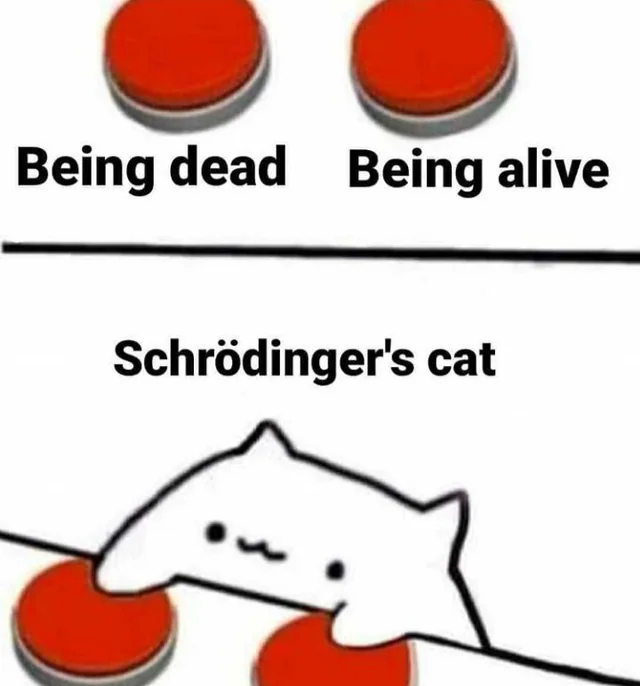
\includegraphics[scale=0.23]{figures/Kommunikation/superposition_schroedinger}
		\end{column}
	\end{columns}
\end{frame}

\begin{frame}
	\frametitle{Superposition \& Qubits II}
	\begin{definition}
		\justifying
		 \enquote{[A] single qubit is in a superposition of two classical bits, [...] the measurement actually only results in one classical bit of information: either 0 or 1.}\cite{Hughes2021}
	\end{definition}
	\begin{definition}
		\justifying
		\textit{Hier muss ich noch in die SLUB} -- \cite{Schumacher1995}
	\end{definition}
\end{frame}

\begin{frame}
	\frametitle{Bloch-Kugel}
	\begin{columns}
		\begin{column}{0.6\linewidth}
			Grafische Darstellung eines Qubit Zustandes\\
			\vspace{0.5em}
			Jeder Punkt auf der Kugel = möglicher Qubit-Zustand\\
			\vspace{0.5em}
			$|\Psi\rangle = \alpha|0\rangle + \beta|1\rangle$\\
			{\centering mit}\\
			$|\alpha^2| + |\beta^2| = 1 \& \alpha, \beta \in {\displaystyle\mathbb{C}}$\\
			\vspace{0.5em}
			Wahrscheinlichkeit:\\
			$|0\rangle$ zu messen = $\alpha^2$\\
			$|1\rangle$ zu messen = $\beta^2$\\
		\end{column}
		\begin{column}{0.39\linewidth}
			\img{0.85\linewidth}{Kommunikation/bloch_sphere}{quantum:bloch_sphere}{Bloch-Kugel}{Bloch-Kugel}
		\end{column}
	\end{columns}
\end{frame}

\begin{frame}
	\frametitle{Verschr{\"a}nkung}
	\begin{columns}
		\begin{column}{0.6\linewidth}
			Zwei oder mehr Teilchen sind so miteinander verbunden (Quantensystem), dass die Messung des Zustands eines Teilchens den Zustand der anderen sofort beeinflusst, unabhängig von der Entfernung
			\vspace{0.5em}
			Bell‘sche Ungleichung:\\
			$S = |E(a,b)-(a,b^{'})+E(a^{'},b)+(a^{'},b^{'})| \leq 2$\\
			$S > 2$, dann Verschränkung
		\end{column}
		\begin{column}{0.4\linewidth}
			\img{0.85\linewidth}{Kommunikation/verschraenkung}{quantum:entanglement}{Veranschaulichung von Quantenverschr{\"a}nkung}{Veranschaulichung von Quantenverschr{\"a}nkung}
		\end{column}
	\end{columns}
\end{frame}

%\begin{frame}{Animated GIF Example}
%	\animategraphics[autoplay,loop,width=0.5\linewidth]{10}{figures/frames/test/frame-}{0}{5}
%\end{frame}
	\section{Quantenkommunikation an Hand eines Beispiels}
\begin{frame}[allowframebreaks]
	
\end{frame}
	\section{Zusammenfassung}
\begin{frame}[allowframebreaks]
	
\end{frame}

	%*************************************************************************
	% Literaturverzeichnis
	%*************************************************************************
	\section{Quellenverzeichnis}
	\begin{frame}[allowframebreaks]
		\frametitle{Quellenverzeichnis}
		\bibliographystyle{baalphadin}
		%		\pdfbookmark[-1]{Quellenverzeichnis}{pdf-Bibliography}%
		%		\phantomsection%
		% BibTeX:
		\bibliography{bibliography}
	\end{frame}
	
\end{document}